\documentclass[report.tex]{subfiles}

\externaldocument{report}

\begin{document}

\section{性能評価}

今回製作できたラジオは,以下のような仕様となった。

\begin{enumerate}
	\item クリスタルイヤホンを用いてアンプなしでラジオを聞くことができた。
	\item 4段のアンプを用いてスピーカーを駆動することができた。
	\item 多少の雑音はあるが、何を話しているのかを聞き取ることができた。
	\item 一号機は、ニッポン放送とTBSラジオと文化放送を受信することが出来たが複数の放送局が同時に聞こえるようになってしまった。
	      二号機は、一号機とほぼ同じ性能だが、音が一号機と比べて小さい。
	      三号機は、全く動作しなかった。
	\item 可変抵抗を用いて音量調整を行うことができた。
	\item 教室(CAD室)内のどこでも受信できたが(TBSラジオと文化放送)、ニッポン放送は窓側でないと聞き取れなかった。
	\item 一号機は、直径24cm、高さ38cmのループアンテナを用いているため、持ち運びが困難であった。
	      二号機は、直径6.5cm、高さ16.5cmのループアンテナを用いているため、持ち運びが容易であった。
	      三号機は、一号機二号機と比べるとかなり小さいが、受信できなかったため使えない。
\end{enumerate}

\subsection{アンテナ}

今回は合計で3つのアンテナを用意した(1号機と2号機は製作したもの、3号機は既製品)。
それぞれの仕様を\wtab{ant}に示す。
また、それぞれの写真を\wfig{1}、\wfig{2}、\wfig{3}に示す。

\begin{table}[H]
	\centering
	\caption{アンテナの各パラメータ}
	\label{tab:ant}
	\begin{tabular}{ccccccc} \hline
		名称  & 直径[mm] & 巻き数[turn] & 抵抗[\(\Omega\)] & 長さ[mm] & コア材質  & コア長[mm] \\ \hline
		1号機 & 240    & 24        & 4.6            & 11     & 空気    & -       \\
		2号機 & 65     & 135       & 0.5            & 50     & 空気    & -       \\
		3号機 & 10     & 70        & 28.0           & 12     & フェライト & 42      \\ \hline
	\end{tabular}
\end{table}

\begin{figure}[H]
	\centering
	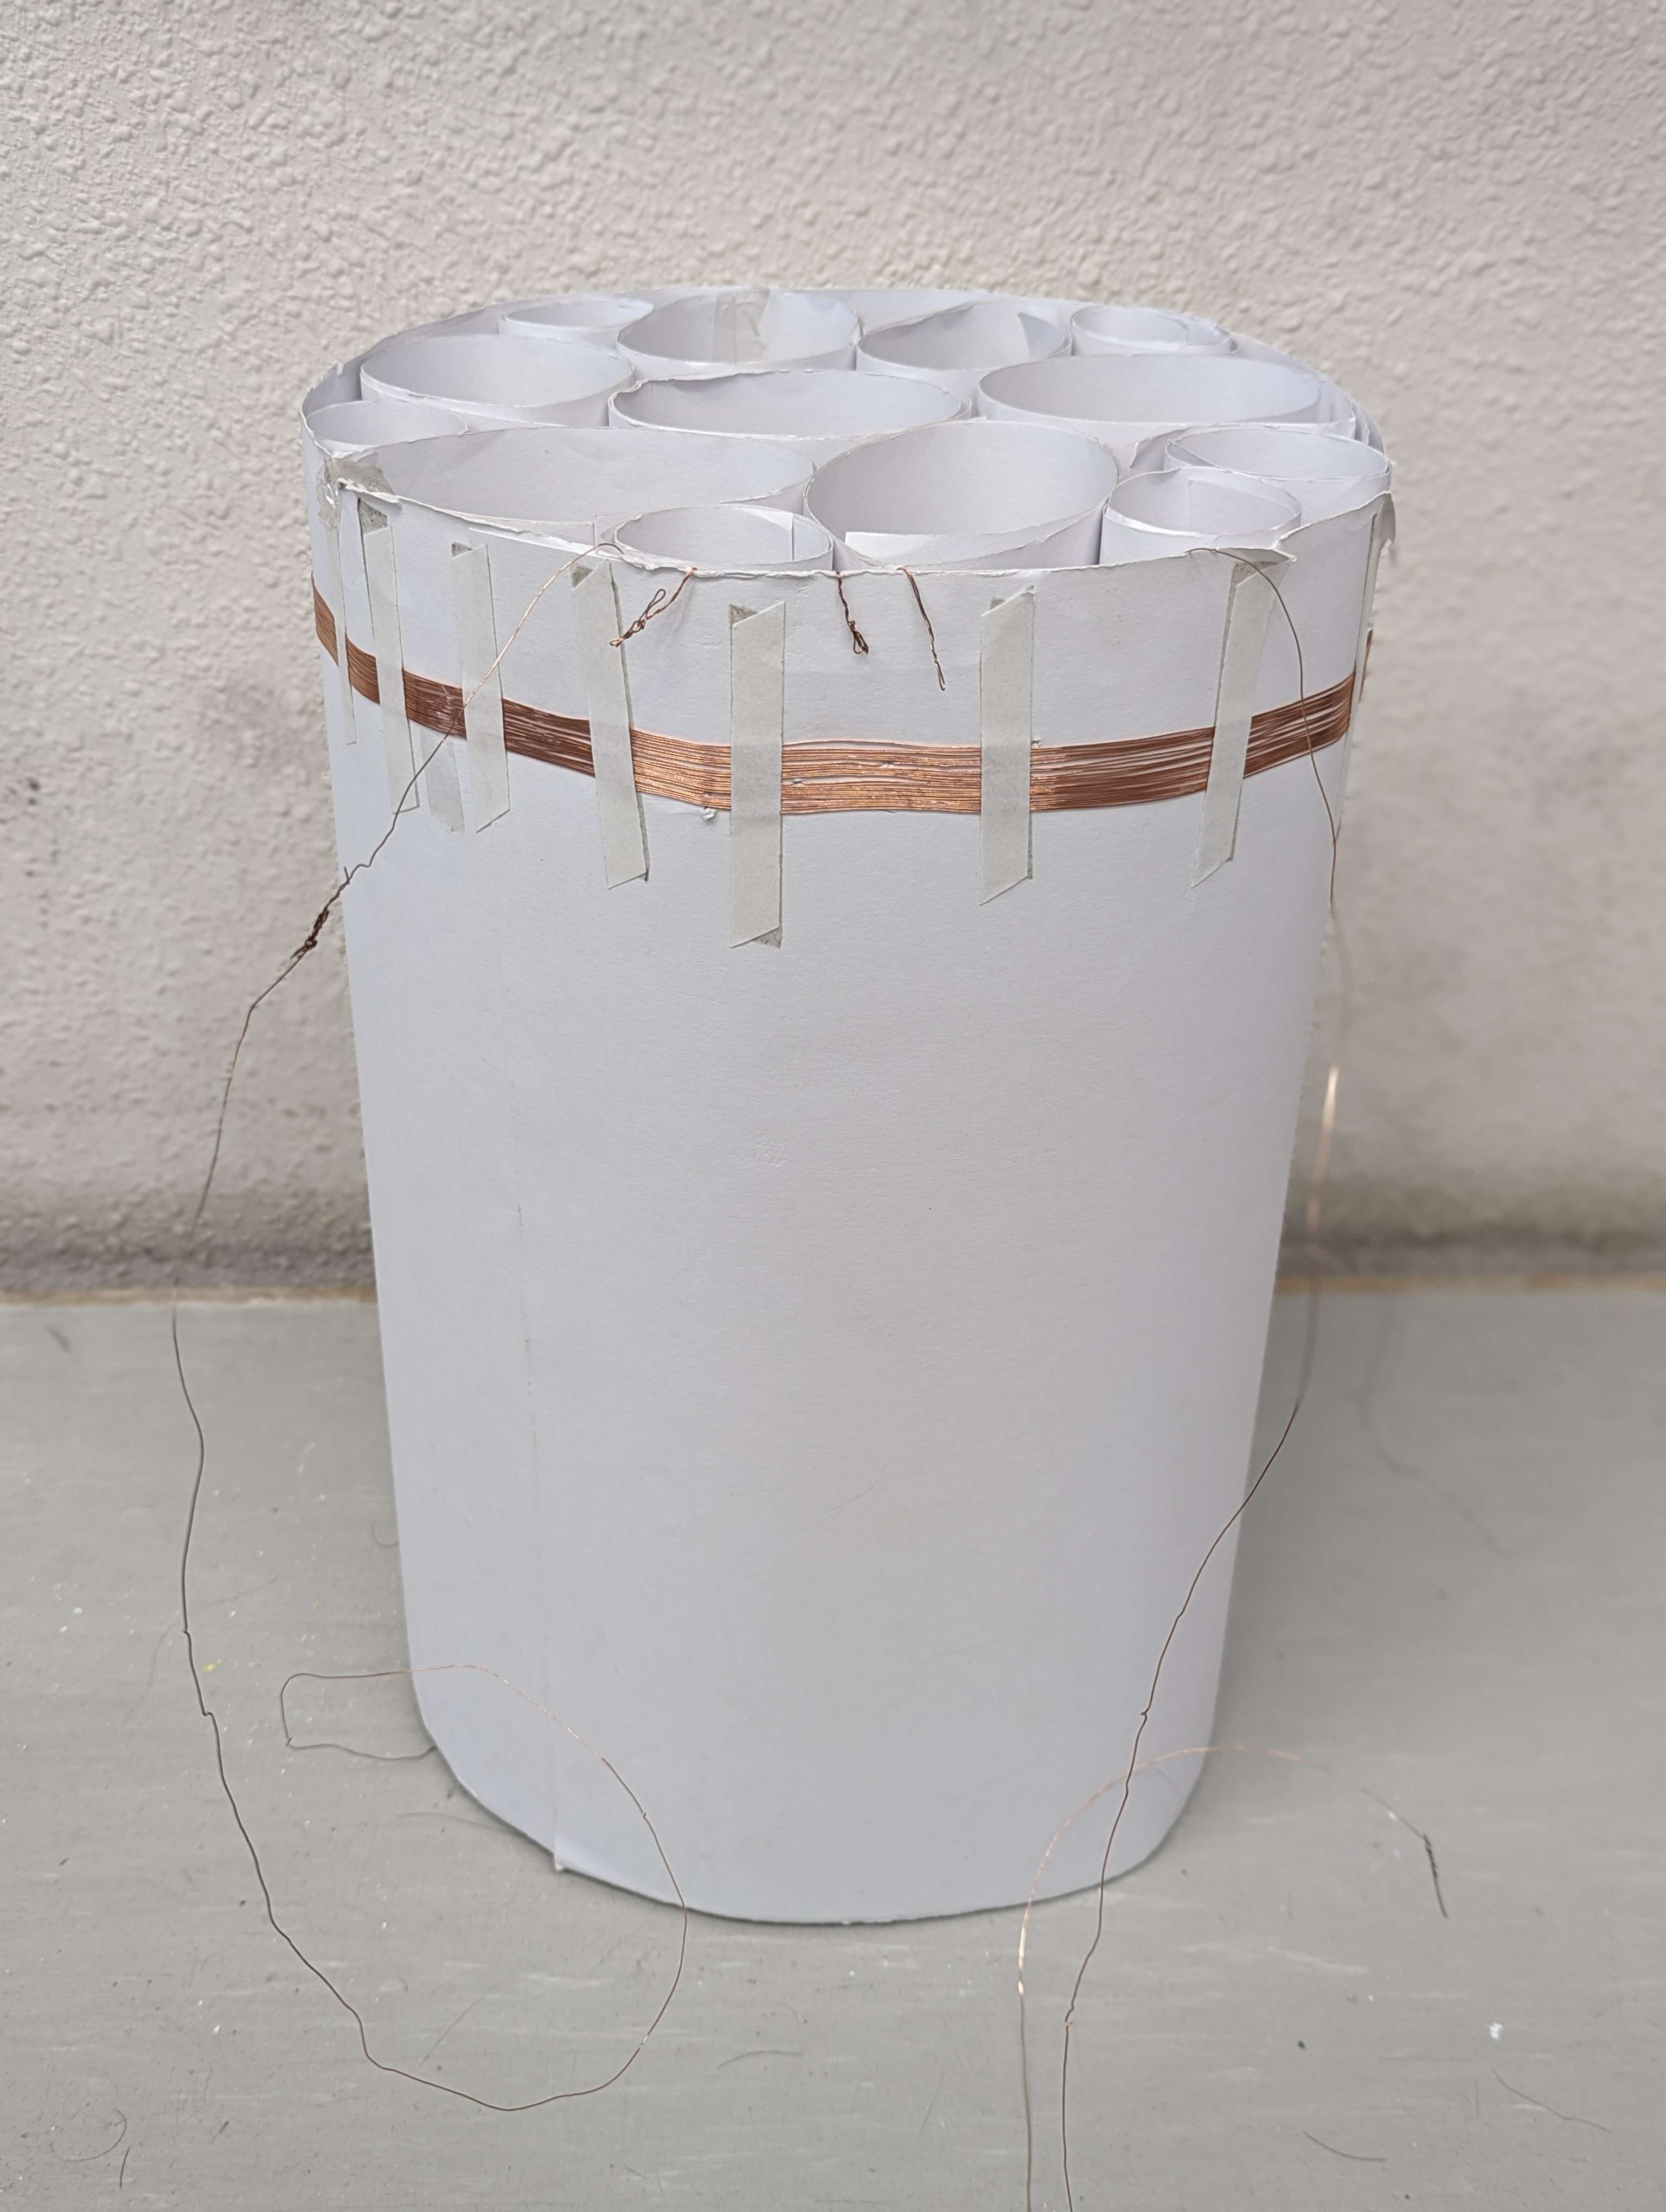
\includegraphics[width=7cm]{fig/1.jpg}
	\caption{アンテナ1号機の写真}
	\label{fig:1}
\end{figure}

\begin{figure}[H]
	\begin{minipage}[b]{0.5\linewidth}
		\centering
		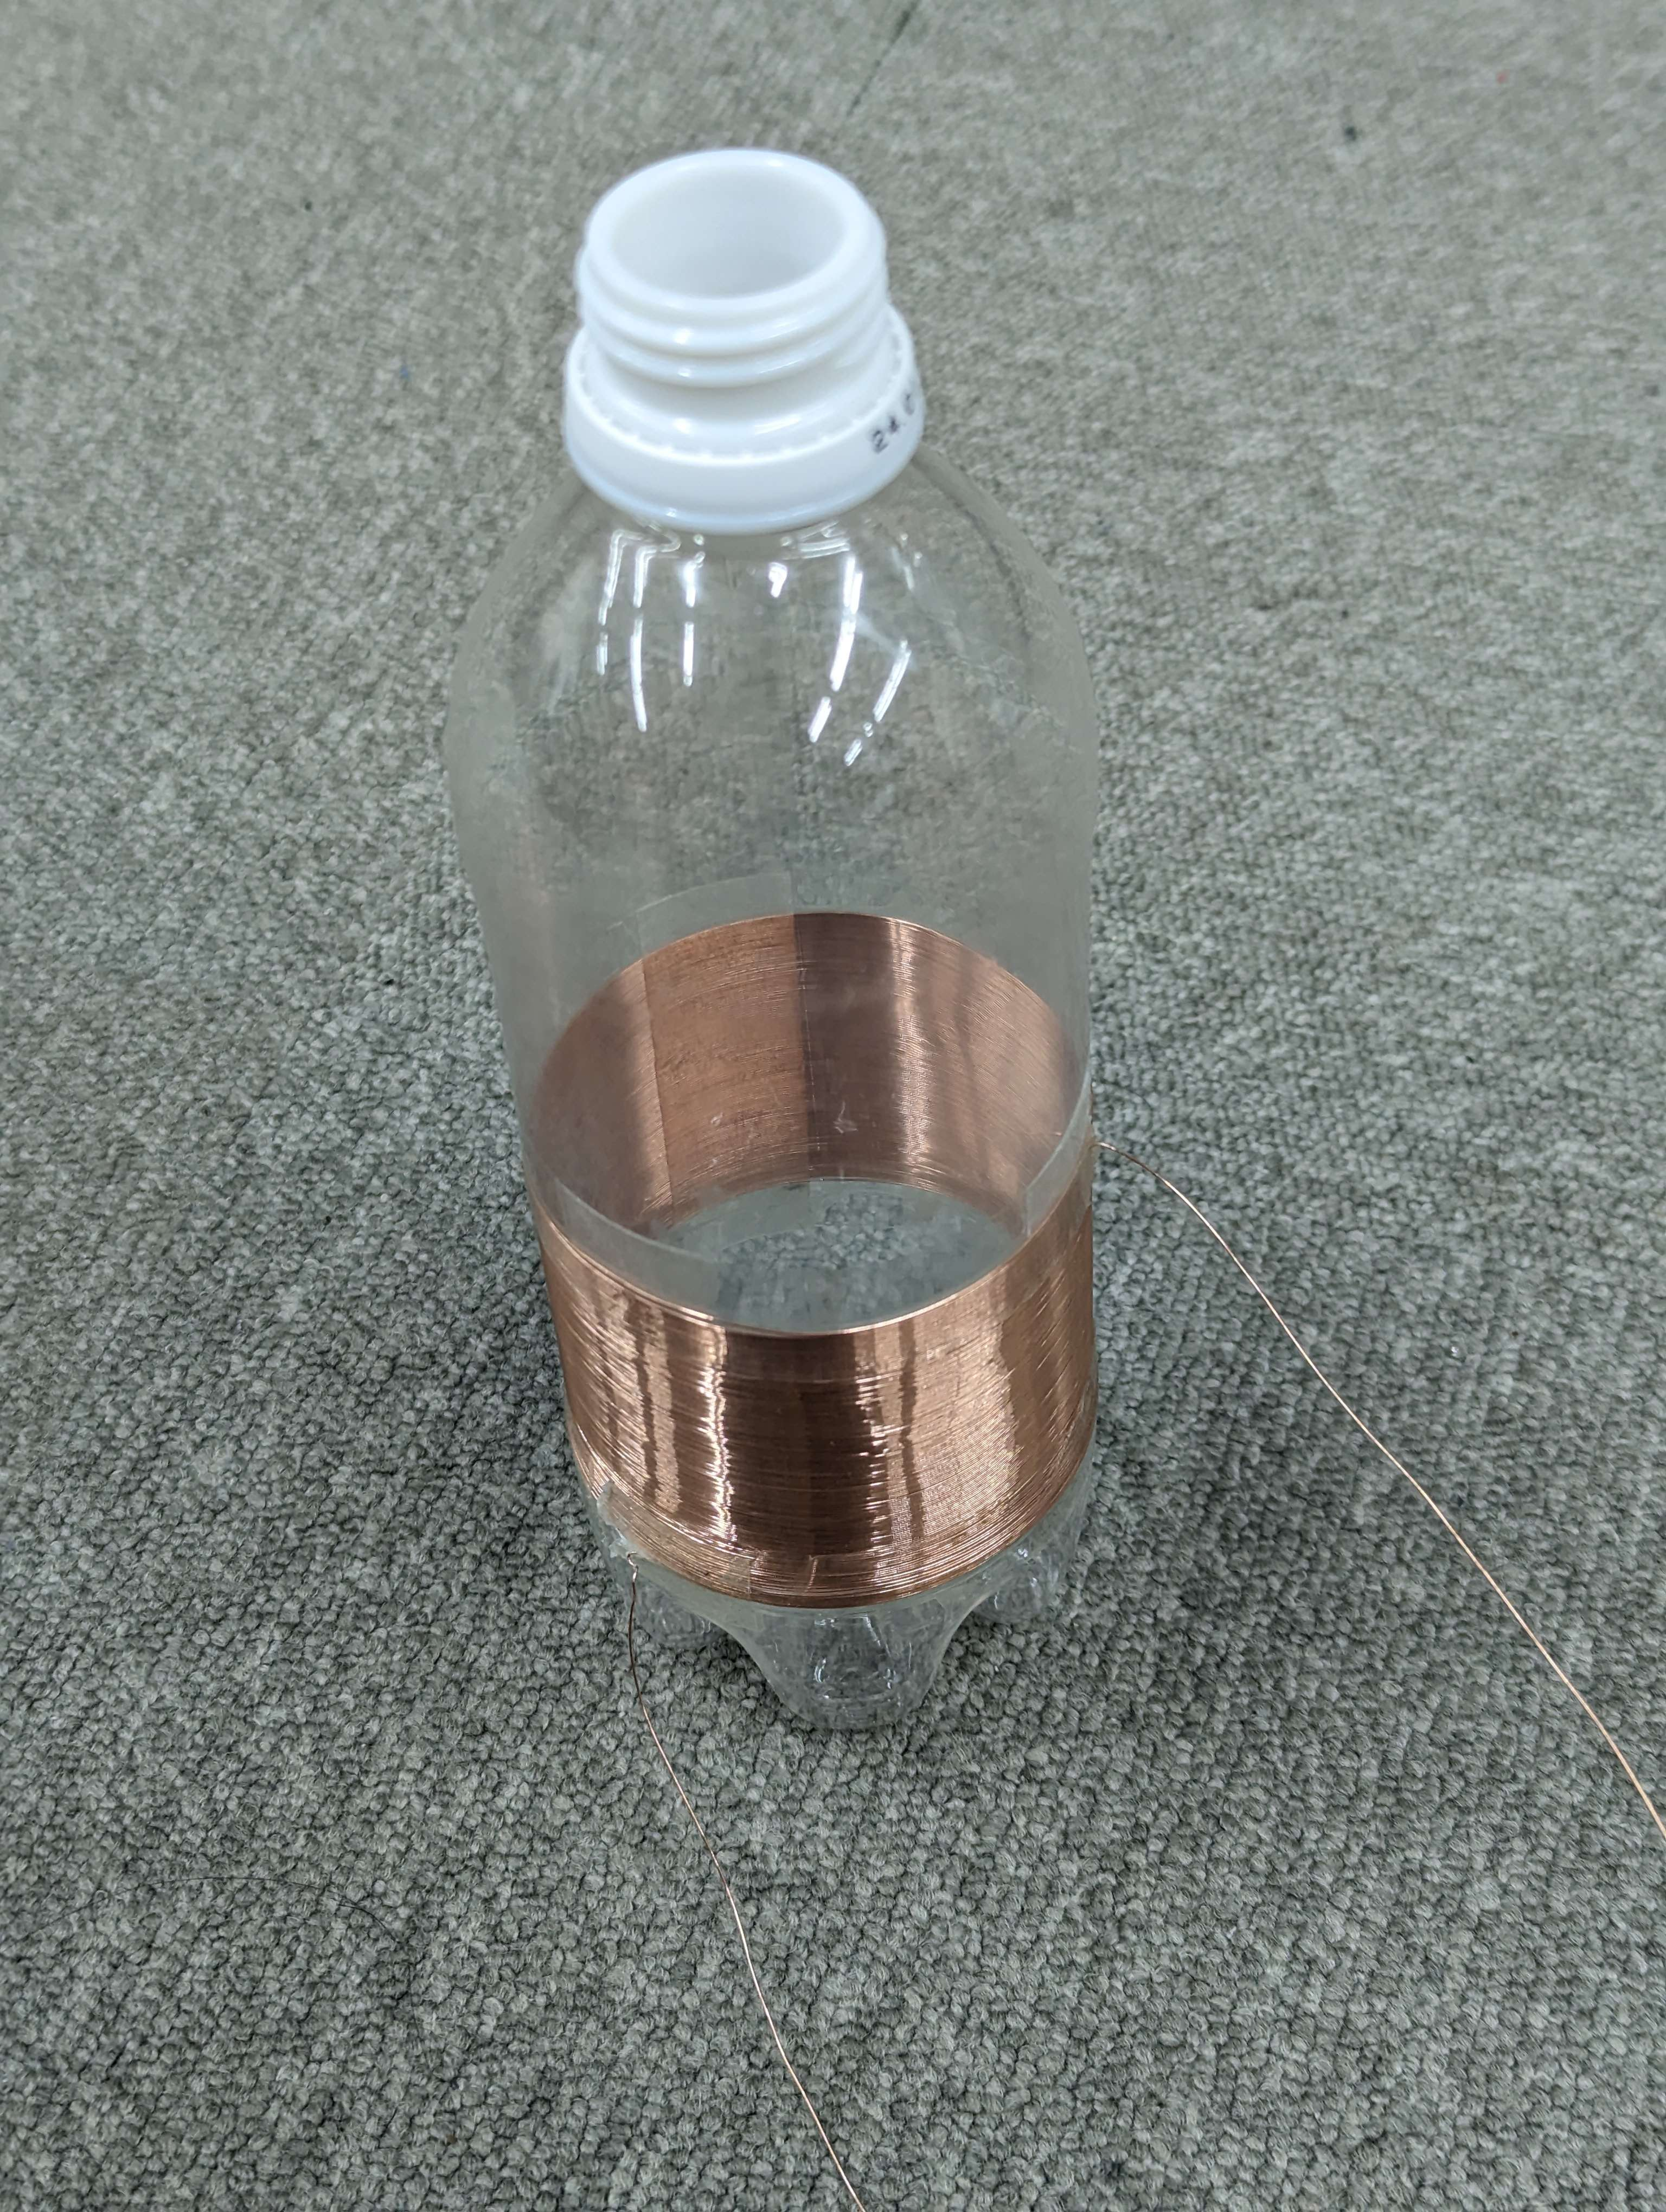
\includegraphics[width=7cm]{fig/2.jpg}
		\caption{アンテナ2号機の写真}
		\label{fig:2}
	\end{minipage}
	\begin{minipage}[b]{0.5\linewidth}
		\centering
		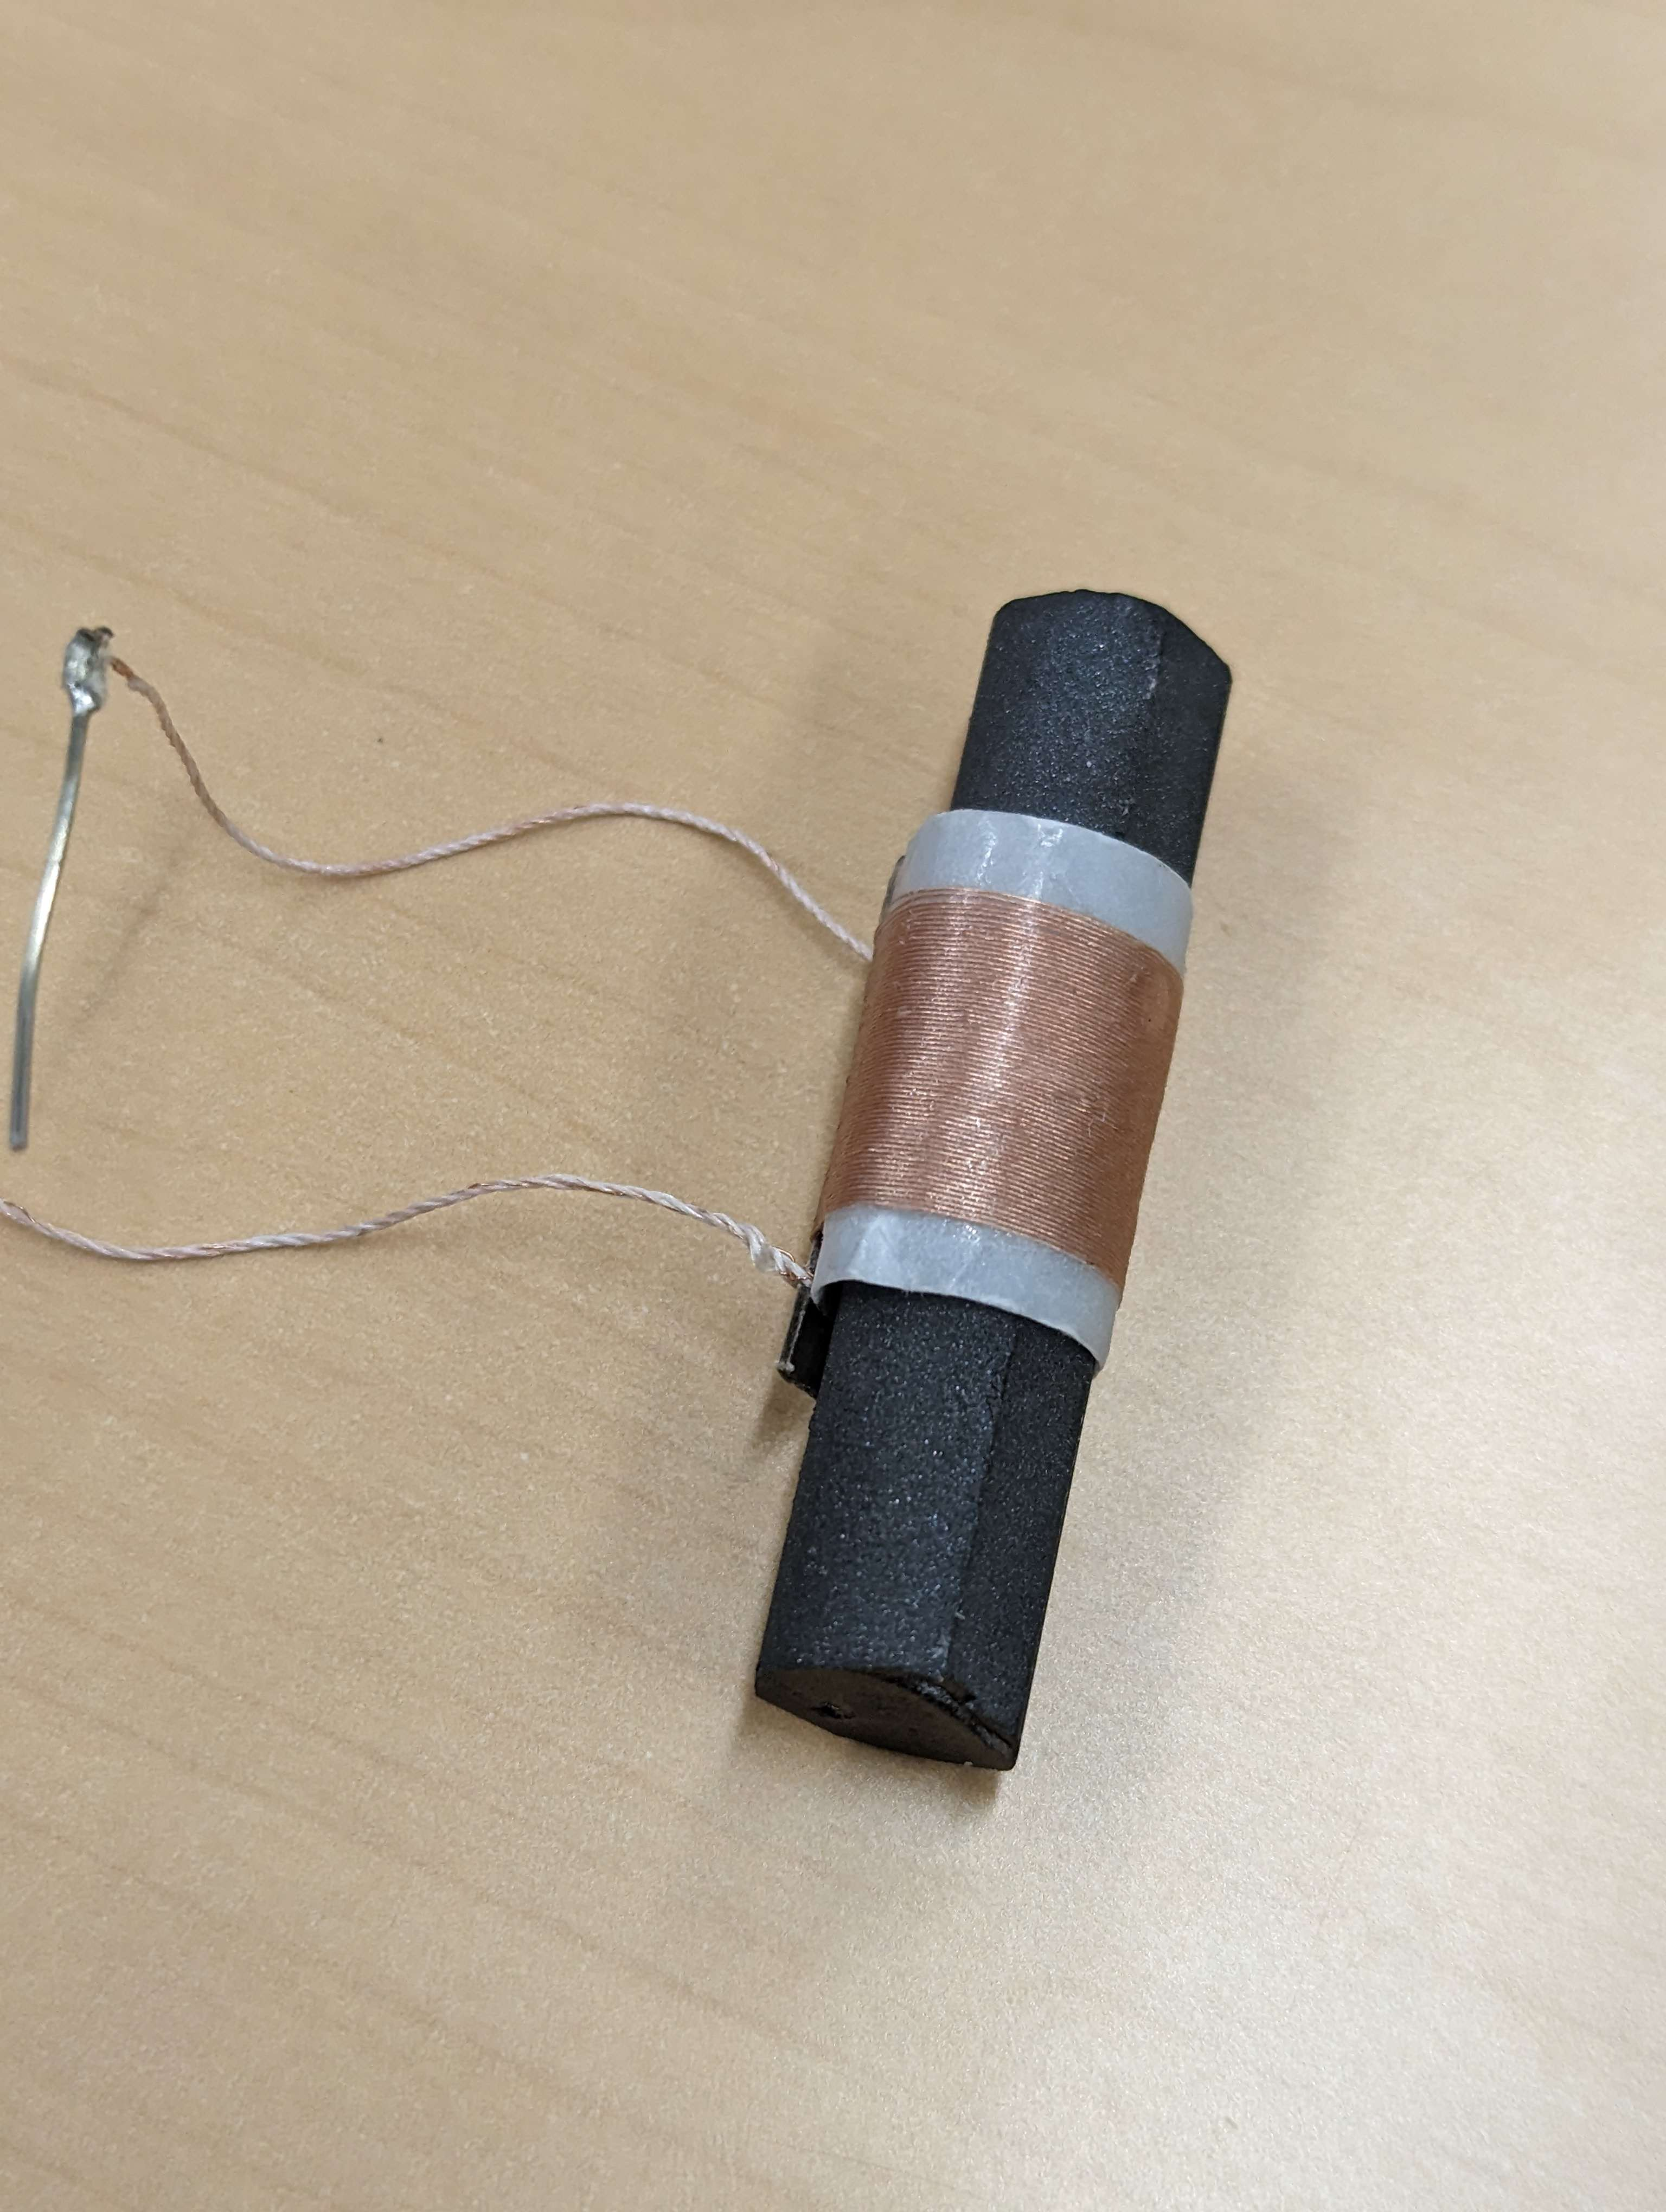
\includegraphics[width=7cm]{fig/3.jpg}
		\caption{アンテナ3号機の写真}
		\label{fig:3}
	\end{minipage}
\end{figure}

まず、受信できる周波数を特定するために、それぞれのインダクタンスを測定した。
LCRメータが機能しなかったため、それぞれのインダクタンスの測定は、\wfig{inda}のような回路を用いて行った。
周波数を変更させて、共振回路間の電圧を測定し、分圧則より共振周波数の場合はインピーダンスがほぼ無限になるため、5Vの電圧が測定できる。
5Vになった周波数から、\weq{resonance}と共振回路内のセラミックコンデンサ150 pFの値を用いて、インダクタンスを計算した。

\begin{figure}[H]
	\centering
	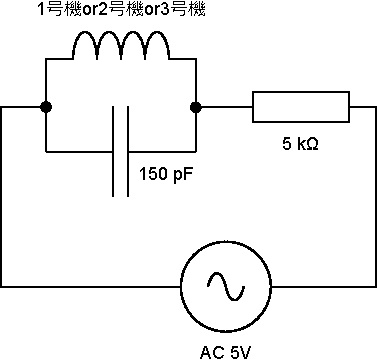
\includegraphics[width=8cm]{fig/inda.pdf}
	\caption{インダクタンス測定回路}
	\label{fig:inda}
\end{figure}

\wfig{inda2}に、\wfig{inda}の測定結果を示す。
1号機(Unit1)と2号機(Unit2)は5.00 Vが計測できたが、3号機(Unit3)は4.31 Vまでしか計測できなかった。
また、\wfig{inda2}には載せていないが、3号機のフェライトを抜いたら共振しなくなり、0 Vが観測された。

\begin{figure}[H]
	\centering
	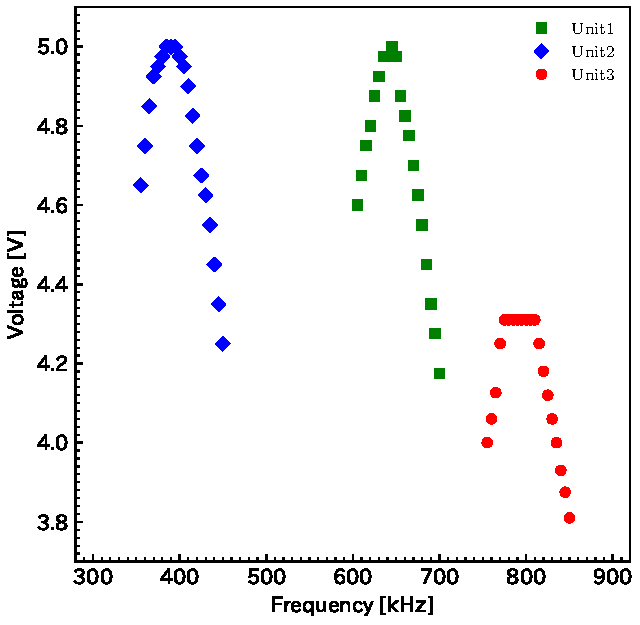
\includegraphics[width=10cm]{fig/inda_inda.pdf}
	\caption{インダクタンス測定回路の共振}
	\label{fig:inda2}
\end{figure}

\wfig{inda2}の結果から、\wtab{ant2}のように、インダクタンスと受信できる周波数を計算した。
受信できる周波数は、\wfig{radio-circuit}の4 pF \(\sim\) 260 pFのバリアブルコンデンサ(CBM-113B-1C4)を用いることを想定している。

\begin{table}[H]
	\centering
	\caption{インダクタンス測定回路の結果}
	\label{tab:ant2}
	\begin{tabular}{ccccc} \hline
		名称  & 最大電圧[V] & 共振周波数[kHz] & インダクタンス[\(\upmu\)H] & 受信できる周波数[kHz](理論上)        \\ \hline
		1号機 & 5.00    & 約645       & 405.91              & 約 489.91 \(\sim\) 3949.80 \\
		2号機 & 5.00    & 約390       & 1110.24             & 約 296.23 \(\sim\) 2388.26 \\
		3号機 & 4.31    & 約790       & 270.58              & 約 600.69 \(\sim\) 4842.93 \\ \hline
	\end{tabular}
\end{table}

\wtab{ant2}より、一号機と二号機は\wtab{zyushin}の全ての局を聞くことができるのではないかと考えた。
しかし、綺麗に聞くことができなかったため、バリアブルコンデンサが機能していないのではないかと考えた。
そこで、今度は\wfig{inda3}のようにインダクタンスを一号機に固定させて、バリアブルコンデンサの容量を変化させて、受信できる周波数を測定した(こちらもLCRメータが機能しなかった)。
バリアブルコンデンサのつまみを最小にしたときと最大にしたときの二種類を測定した。

\begin{figure}[H]
	\centering
	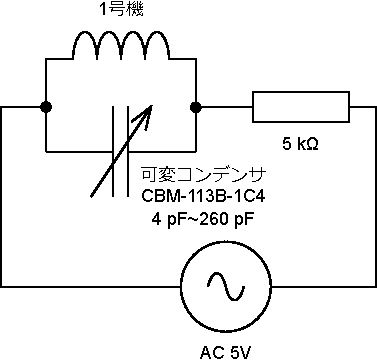
\includegraphics[width=8cm]{fig/inda3.pdf}
	\caption{バリアブルコンデンサ測定回路}
	\label{fig:inda3}
\end{figure}

\wfig{inda4}に、\wfig{inda3}の測定結果を示す。また\wtab{Q}に,各条件でのQ値を示す。2号機つまみ最大に関しては,測定点が足りずQ値を算出できなかった。
正規化Q値は\weq{sQ}より算出した。

\begin{table}[H]
	\centering
	\caption{共振回路のQ値(max:つまみ最大,min:つまみ最小)}
	\label{tab:Q}
	\begin{tabular}{ccccccc} \hline
		     & \(A_0\) & \(f_0\) & \(\omega_1\) & \(\omega_2\) & Q値     & 正規化Q値  \\ \hline
		1min & 4.68    & 495     & 450          & 550          & 0.0468 & 23.166 \\
		1max & 3.54    & 1350    & 955          & 1725         & 0.0046 & 6.206  \\
		2min & 4.89    & 300     & 251          & 358          & 0.0457 & 13.710 \\
		2max & 3.04    & 890     & -            & -            & -      & -      \\ \hline
	\end{tabular}
\end{table}

\begin{align}
	正規化Q値 =Q値/f_0 \label{eq:sQ}
\end{align}

バリアブルコンデンサのつまみを最小(min)にした場合は、Q値が高かった。
しかし、バリアブルコンデンサのつまみを最大(max)にした場合は、Q値が低かった。
このため、バリアブルコンデンサのつまみを最大にした場合は、\wtab{ant2}の1200 kHz付近の局が全て聞こえてしまう。
実際のところTBSラジオと文化放送が混ざって聞こえてしまった。

\begin{figure}[H]
	\centering
	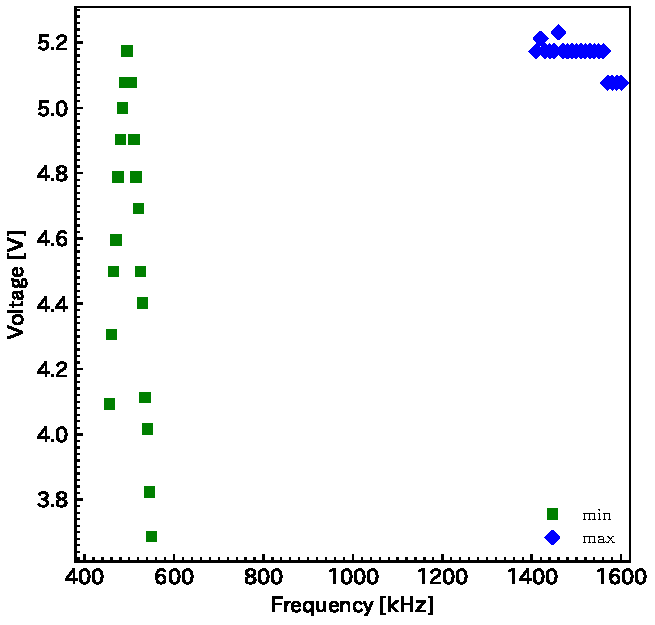
\includegraphics[width=8cm]{fig/min_max.pdf}
	\caption{バリアブルコンデンサ測定回路の共振}
	\label{fig:inda4}
\end{figure}

\begin{figure}[H]
	\centering
	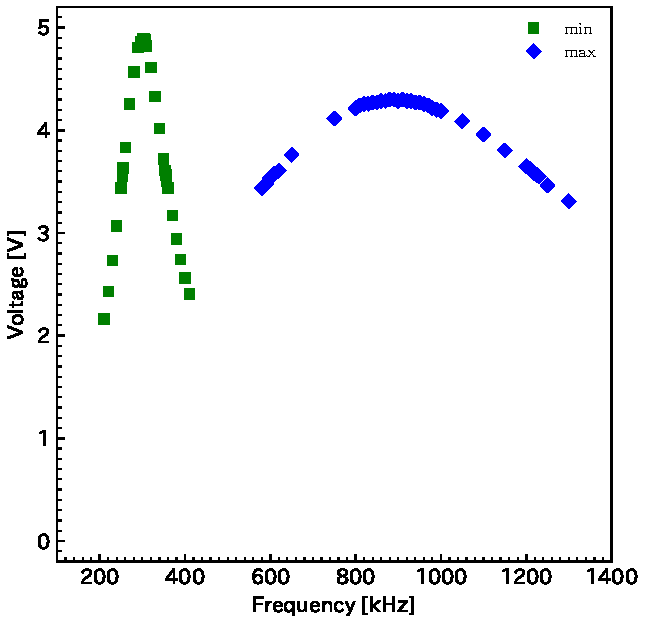
\includegraphics[width=8cm]{fig/min_max2.pdf}
	\caption{バリアブルコンデンサ測定回路の共振}
	\label{fig:inda5}
\end{figure}



\wtab{ant3}に、\wfig{inda4}の結果から、バリアブルコンデンサの最小と最大を計算した。
maxの共振周波数は、Q値が低かったため判断が難しかったが、最大電圧が出力された周波数を共振周波数とした(オシロスコープの分解能のせいであまり正確な値は取れなかった)。
\wtab{ant3}より、バリアブルコンデンサのつまみを最小にしたときは、理論上の値と実際の値がかなり異なっている。
しかし、\wtab{ant2}のに出ているすべての局を聞くことができる。

\begin{table}[H]
	\centering
	\caption{バリアブルコンデンサ測定回路の結果}
	\label{tab:ant3}
	\begin{tabular}{cccccc} \hline
		つまみ & 最大電圧[V] & 共振周波数[kHz] & 理論上の値[pF] & 実際の値[pF] \\ \hline
		min & 5.17    & 約495       & 260       & 254.7    \\
		max & 5.23    & 約1460      & 4         & 29.3     \\ \hline
	\end{tabular}
\end{table}

この値を用いて、もう一度\wtab{ant2}の受信できる周波数を計算した。
それを\wtab{ant5}に示す。
\wtab{ant5}より、二号機の受信できる周波数は、\wtab{zyushin}よりかなり狭いことがわかる。

\begin{table}[H]
	\centering
	\caption{実際に受信できる周波数帯}
	\label{tab:ant5}
	\begin{tabular}{ccccc} \hline
		名称  & インダクタンス[\(\upmu\)H] & 受信できる周波数[kHz](理論上)      & 受信できる周波数[kHz](実際)       \\ \hline
		1号機 & 405.91              & 489.91 \(\sim\) 3949.80 & 約 495.0 \(\sim\) 1460.0 \\
		2号機 & 1110.24             & 296.23 \(\sim\) 2388.26 & 約 299.3 \(\sim\) 882.4  \\
		3号機 & 270.58              & 600.69 \(\sim\) 4842.93 & 約 606.3 \(\sim\) 1787.5 \\ \hline
	\end{tabular}
\end{table}

\wtab{ant5}より、受信できる周波数は一号機はほとんど聞くことができ(ラジオの放送局数的に)、二号機は半分ほど聞くことができ、三号機はほとんど聞くことができない(こちらはそもそも同調回路として機能しているのか分からない)。
特に、NHKなどは全く聞くことができなかった。
原因として、そもそも電波が届いていないのではないかと考えた。
レーダー方程式によって求めた電力密度と、教室から送信局までの方角を\wtab{aaa}に示す。

\begin{table}[H]
	\centering
	\caption{それぞれの電力密度と方角}
	\label{tab:aaa}
	\begin{tabular}{ccc} \hline
		放送局    & 電力密度[\(\rm{W/km^2}\)] & 方角(窓は東) \\ \hline
		NHK第1  & 8.63                  & 北北西     \\
		NHK第2  & 14.38                 & 北北西     \\
		AFN    & 7.93                  & 北北西     \\
		TBSラジオ & 14.29                 & 北北西     \\
		文化放送   & 13.48                 & 北北西     \\
		ニッポン放送 & 7.87                  & 南東      \\
		ラジオ日本  & 65.40                 & 南西      \\ \hline
	\end{tabular}
\end{table}

今回ではTBSラジオ、文化放送、ニッポン放送(こちらは窓に近づけないと聞こえない)が聞くことができた。
TBSラジオと文化放送は、電力密度が14 \(\rm{W/km^2}\)ほどであり、電力密度が他のものと比べて高い。
方角も北北西であり、辛うじて電波が受信できそうな方角である。
ラジオ日本が聞こえなかった原因は、方角的に壁が邪魔をしているのではないかと考えられる。
逆に電力密度が低いラジオ日本で壁に近づけたら聞こえたのは、南東なので方角的に受信しやすかったのではないかと考えられる。
また、NHK第1とAFNは、電力密度が低いので聞くことができなかったと考えられる(方角も北北西で微妙)。
疑問として、NHK第2は方角も電力密度もTBSラジオとほとんど変わらないのに聞こえなかったこと。
ラジオ日本は、方角が悪いが、電力密度は他の送信所に比べて極端に高いのにも関わらず、聞こえなかったことである。

\subsection{検波}

\wfig{koil}に、ループアンテナアンテナから取り出された電圧を示す。
\wfig{koil_diode}に、\wfig{koil}から取り出された電圧を検波回路で検波された電圧を示す。
\wfig{koil_diode_bi}に、\wfig{koil_diode}からカップリングコンデンサを通して取り出された電圧を示す。
関係ないかもしれないが、\wfig{koil}\wfig{koil_diode}\wfig{koil_diode_bi}すべてオシロスコープの分解能の影響で決まった値しか検出できなかった。
\wfig{koil}より、ノイズと思われる部分を含めないで、最大約0.02[V]の電圧が観測された。
\wfig{koil_diode}より、逆電圧がほとんどないため、ゲルマニウムダイオードの整流作用が働いていることが確認できる。
また、\wfig{koil_diode_bi}より、\wfig{koil_diode}の直流成分(0.01[V]ぐらい)がカットされていることがわかる。
そのため、検波回路は正常に動作していると考えられる。

\begin{figure}[H]
	\centering
	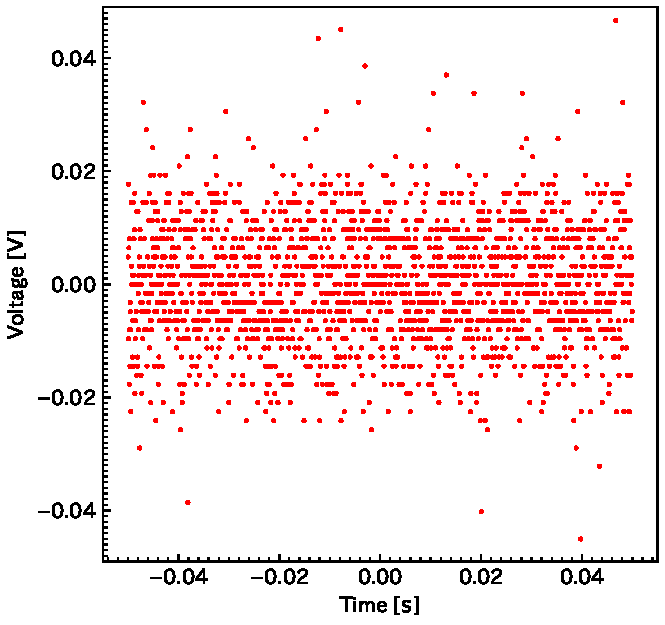
\includegraphics[width=7cm]{fig/koil.pdf}
	\caption{ループアンテナから取り出された電圧}
	\label{fig:koil}
\end{figure}

\begin{figure}[H]
	\begin{minipage}[b]{0.5\linewidth}
		\centering
		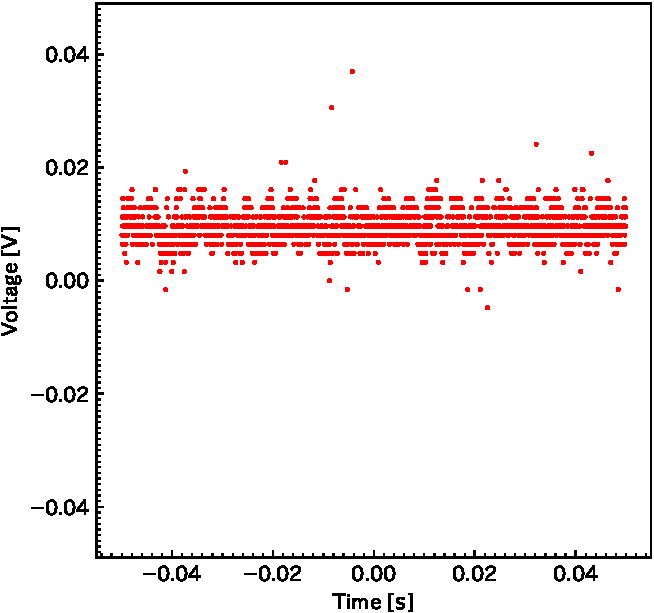
\includegraphics[width=7cm]{fig/koil_diode.pdf}
		\caption{検波回路で検波された電圧}
		\label{fig:koil_diode}
	\end{minipage}
	\begin{minipage}[b]{0.5\linewidth}
		\centering
		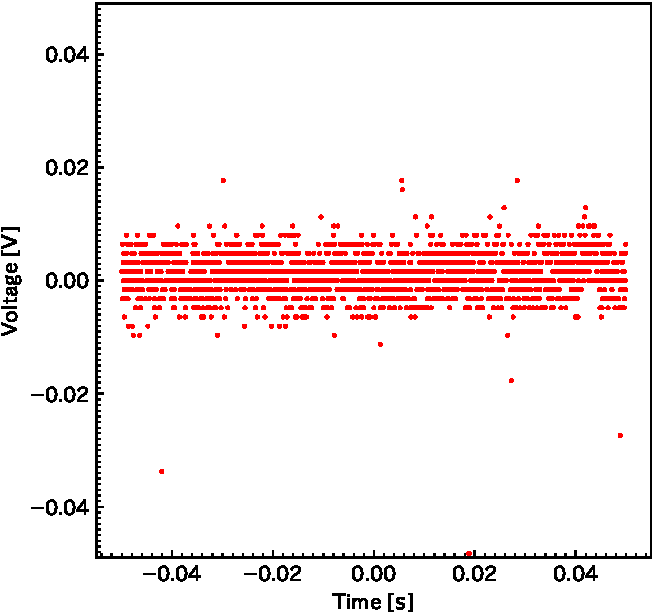
\includegraphics[width=7cm]{fig/koil_diode_bi.pdf}
		\caption{カップリングコンデンサを通したときの電圧}
		\label{fig:koil_diode_bi}
	\end{minipage}
\end{figure}

\subsection{アンプ}

\wfig{gain}に、今回用いた増幅回路のゲイン線図を示す。
\wfig{gain}のTheoretical valueが理想値(5.7倍、15.1175[dB])である。
Lowest rangeが人間が聞こえる周波数の最低値(20[Hz])である。
Highest rangeが人間が聞こえる周波数の最高値(20000[Hz])である。
測定値は、オシロスコープから取り出した波形のCSVファイルから最大値を取り出したものなので、
ノイズなどでゲインが少し理想値よりも高くなっている。
\(10^6\)[Hz]付近で、リップルが発生しており、その後に急激に減少している。
しかし、この領域は人間が聞こえる周波数の範囲外のため、問題ないと考えられる。
逆に、人間が聞こえる周波数の範囲内は、理想値に近い値を取っているため良いと考えられる。

\begin{figure}[H]
	\centering
	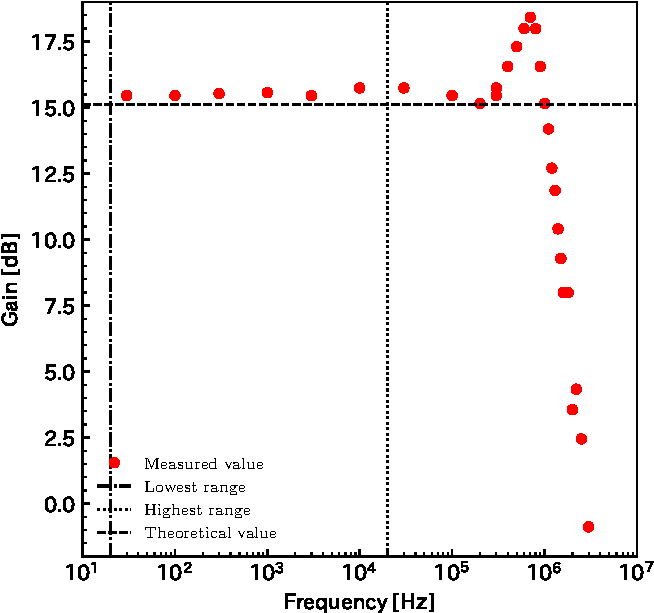
\includegraphics[width=10cm]{fig/gain.pdf}
	\caption{アンプのゲイン線図}
	\label{fig:gain}
\end{figure}

\wfig{12_100m}に100mVの正弦波を入力したときのアンプ一段二段の出力電圧を示す。
アンプ一段では5.7(\(5.7^1\))倍、アンプ二段では32.49(\(5.7^2\))倍に増幅される想定で、実際にそのぐらいの付近まで増幅されている。
また、ノイズがほとんど乗っていないことがわかる。
そのため、アンプは正常に動作していると考えられる。
実際にアンプ一段二段を用いてラジオを聞いたところ、音は小さいがかなりクリアに聞き取ることができた。

\begin{figure}[H]
	\centering
	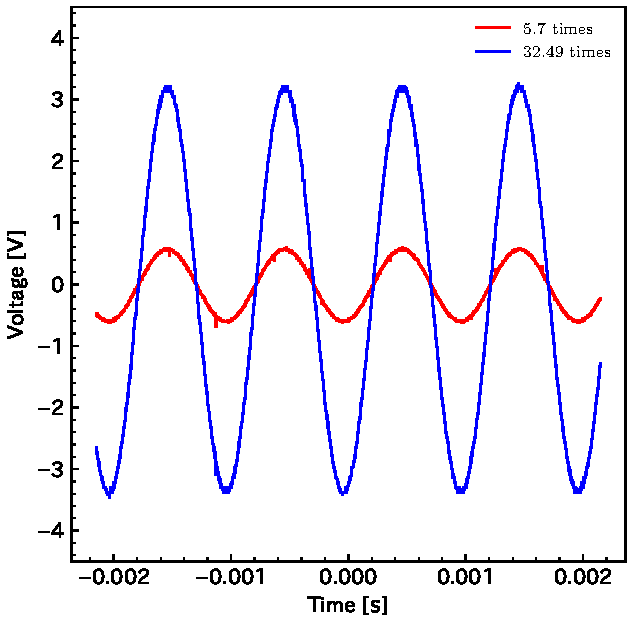
\includegraphics[width=10cm]{fig/level12_100m.pdf}
	\caption{100mVの正弦波を入力したときのアンプ一段二段の出力電圧}
	\label{fig:12_100m}
\end{figure}

\wfig{34_100m}に100mVの正弦波を入力したときのアンプ三段四段の出力電圧を示す。
アンプ三段では185.193(\(5.7^3\))倍に増幅される想定で、\(\pm\)7 V付近で飽和している。
アンプ四段では1055.6001(\(5.7^4\))倍に増幅される想定で、-7,+8 V付近で飽和している。
飽和している原因として、オペアンプの電源が9 Vなので、そこで限界が来たのではないかと考えられる。
アンプ四段はアンプ三段に比べて0.5 Vほどバイアス電圧(電圧の直流成分)が発生していることがわかる。
飽和している部分を見ると、\wfig{12_100m}と比較して、ノイズが増えている。
これは、アンプが増えたことによって、アンプによって発生するノイズが増えたためだと考えられる。

\begin{figure}[H]
	\centering
	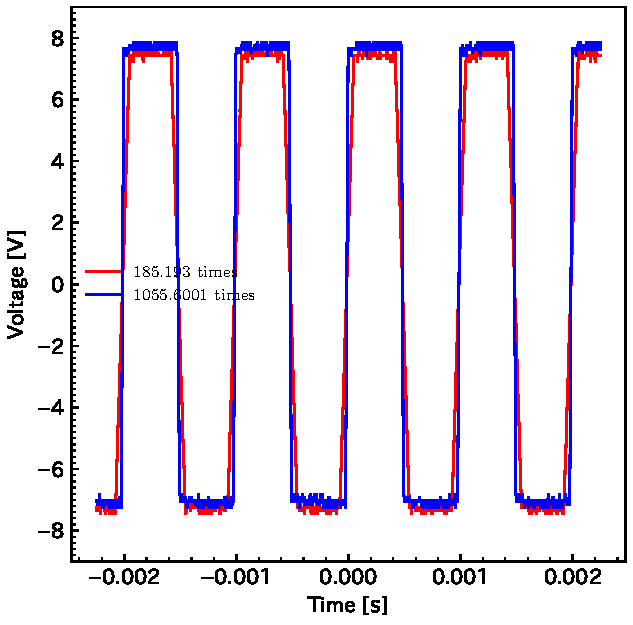
\includegraphics[width=10cm]{fig/level34_100m.pdf}
	\caption{100mVの正弦波を入力したときのアンプ三段四段の出力電圧}
	\label{fig:34_100m}
\end{figure}

\wfig{34_100m}では、入力電圧が高かったため、飽和してしまった。
正弦波の全体を見るために、1mVの正弦波を入力したときのアンプ三段四段の出力電圧を\wfig{34_1m}に示す。
アンプ三段目、四段目共に、ノイズが激しく、正弦波の外形は見えるが、最大値を読むとき、正確な値は計測できない。
大まかにみると、アンプ三段の最小電圧は約-0.2 V、最大電圧は約0.4 Vである。
アンプ四段の最小電圧は約-1 V、最大電圧は約2 Vである。
両方とも、バイアス電圧が発生していることがわかる。
また、両方とも電圧の増幅率はおおよそ正しいように見える。
アンプ三段よりもアンプ四段の方が、ノイズが大きいが、これは三段目までのノイズが四段目で増幅されたためだと考えられる。

\begin{figure}[H]
	\centering
	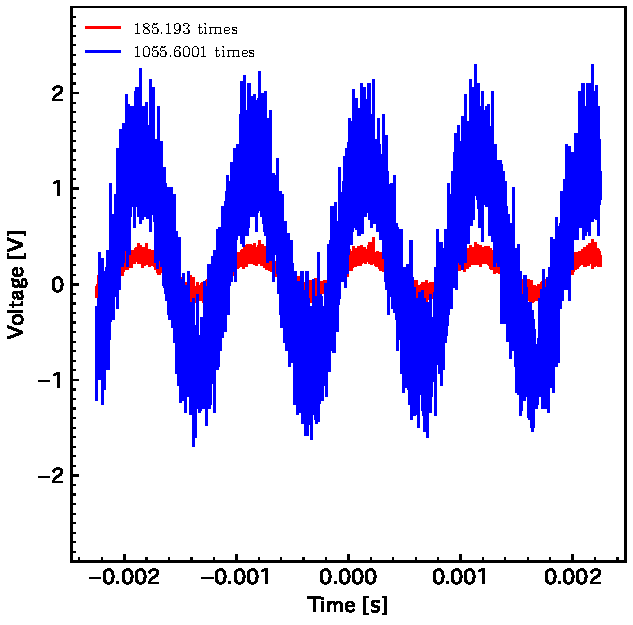
\includegraphics[width=10cm]{fig/level34_1m.pdf}
	\caption{1mVの正弦波を入力したときのアンプ三段四段の出力電圧}
	\label{fig:34_1m}
\end{figure}

\subsection{音量調整}

音量調整は、10 k\(\Omega\)Aカーブの可変抵抗を用いて行った。
\wfig{resi}に、改変抵抗の抵抗値と、そのときの電圧の関係を示す。
\wfig{resi}より、抵抗値が大きくなるにつれて、比例的に電圧が小さくなっていることがわかる。
そのため、可変抵抗を用いて音量調整がしっかりと行われていることがわかる。
実際に、可変抵抗を回して音量調整を行ったところ、音量が変化することが確認できた。

\begin{figure}[H]
	\centering
	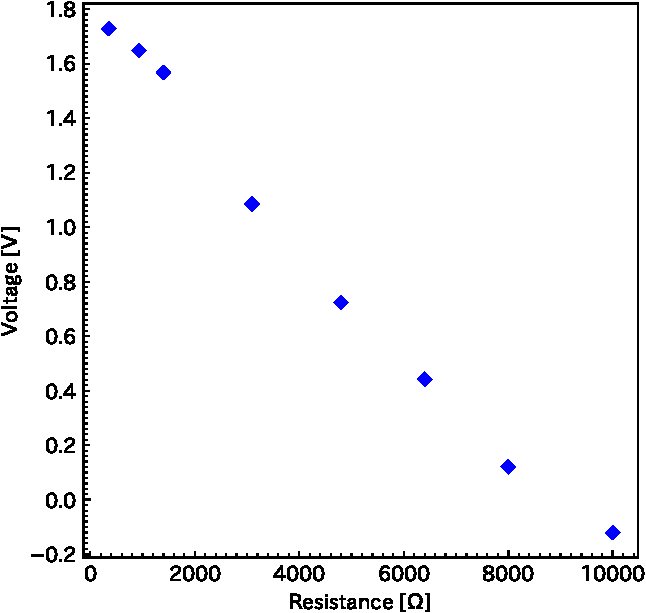
\includegraphics[width=10cm]{fig/resi.pdf}
	\caption{音量調節が出来ているか}
	\label{fig:resi}
\end{figure}

\end{document}
